\section{Candidates}
\par
With there being a plethora of evidence that ``something is there", we can turn our attention to what it might be.
From the observations, we can say that any potential candidate for dark matter must be:
\begin{itemize}
    \item Weakly, or not interacting via electromagnetism;
    \item Weakly, or not interacting via the strong force;
    \item Have some kind of clustering; either by being slow moving (cold) or some other way;
    \item Not baryonic matter;
    \item Stable over the timescale of the universe.
\end{itemize}
There is no limit to the number of candidate particles proposed over the years to describe dark matter; ranging in mass from fractions of a quark to many times the mass of the Sun.
A broad categorisation of these is shown in \autoref{fig:dm_candidates}.
A brief discussion of a selection of these candidates follows along with the current way in which they are being searched for.
It is important to note that dark matter may be a combination of particles.
\begin{figure}[!h]
    \centering
    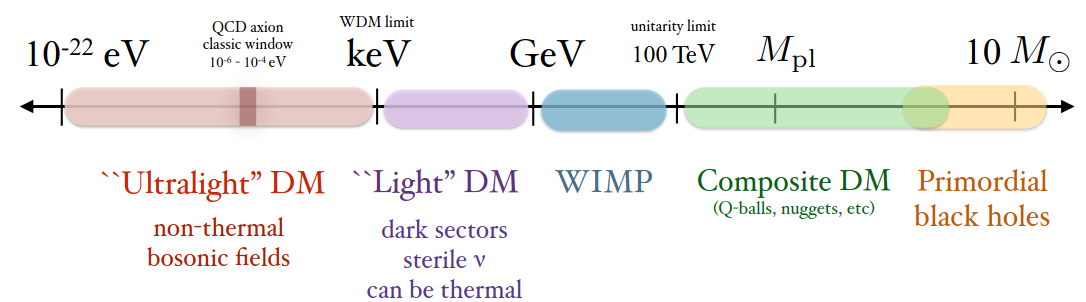
\includegraphics[width=15cm]{Figures/DarkMatterEvidence/dark_matter_candidates.png}
    \caption{Dark matter candidates classified by their approximate mass range. Figure from \cite{dm_figure_candidates_ref}.}
    \label{fig:dm_candidates}
\end{figure}

\subsection{Axions}
\par
Hypothesised in 1977, axions were postulated to solve the strong CP problem of the standard model \cite{axion_origins_ref}.
Axions are pseudo-Goldstone bosons generated by spontaneous symmetry breaking at some energy scale, $f_a$, with the mass of this particle predicted to follow:
\begin{equation}
    m_a \approx (0.6 eV)\frac{10^7 GeV}{f_a}
\end{equation}
The value of $f_a$ is constrained to be greater than that of the electroweak symmetry-breaking scale, given existing constraints.
This leaves a particle with a mass between 10${}^{-6}$ and 10${}^{-2}$ eV which could be dark matter \cite{axions_ref}.
\par
There are multiple possible production mechanisms for axions, such as via thermal production in the early universe.
However, axions produced in this fashion would contribute to hot dark matter \cite{hot_axions_ref}.
Separately, slower, non-relativistic axions can be created through other processes such as the ``re-alignment mechanism" \cite{cold_axion_ref}.
\par
Axions may couple to photons, allowing for conversion to microwaves.
These can be searched for in a microwave cavity with a strong magnetic field applied to it.
In this situation, it is expected that the axion will convert into monochromatic microwave photons.
The ADMX experiment is currently the most sensitive experiment searching for this \cite{admx_experiment_ref}.
\par
Another search for axions is where an axion is absorbed and an atomic electron is ejected.
This electron is then detectable as an electronic recoil.
These searches are typically performed by large underground direct dark matter experiments, with the tightest constraint on axio-electric coupling coming from XENONnT \cite{xenonnt_sr1_er_ref}.
\par
A third approach is via laser beams, whereby a beam is propagated between two superconducting magnets that are optically separated.
If axions are coupling to photons, then the initial beam of photons will transform into axions and then later convert back, allowing the light to be seen through the optical barrier.
Though not as sensitive as the other axion-photon conversion approaches, it does not have the same uncertainties associated with astrophysics and cosmology.
Two notable experiments using this approach are ALPS \cite{alps_axion_result_ref}, and OSQAR \cite{osqar_axion_result_ref}. 
\par
Other search methods are also being explored such as axion induced nuclear electric dipole moment (see CASPEr \cite{casper_experiment_ref}), axion to X-ray conversion in the presence of a magnetic field (see IAXO \cite{iaxo_experiment_ref}), and energy-loss in galactic observables such as supernova explosions due to axion-electron coupling \cite{axions_from_supernova_ref}.

\subsection{Neutrinos}
\par
One of the first candidates suggested as dark matter were neutrinos: the stable, long-lived and weakly-interacting particles in the standard model.
Unfortunately, N-body simulations have shown that these standard model neutrinos are inconsistent with galactic structural formations that are observed \cite{neutrinos_and_galaxy_clustering_ref}. 
This has not ruled out neutrinos entirely, with a new species suggested that interacts only gravitationally, namely sterile neutrinos \cite{sterile_neutrinos_ref}.
Postulated to have a small mixing angle with standard model neutrinos, this would allow for limited interaction between this dark matter and standard model matter.
\par
The most recent excitement around this is an unidentified 3.55 keV line in X-ray spectra from several galactic clusters with high dark matter content \cite{sterile_neutrino_xray_decay_ref}.
Decays of sterile neutrinos are a possible explanation for this, though it is still very much up for debate \cite{xray_from_sterile_neutrons_2_ref, xray_from_sterile_neutrons_3_ref}.
The BEST experiment has also pointed towards sterile neutrinos to account for the deficit observed in germanium isotope production \cite{best_sterile_neutrino_result_ref,best_sterile_neutrino_2_ref}.
Other indications of sterile neutrinos came from MiniBooNE, where an excess in neutrino oscillations was observed.
The successor, MicroBooNE, has not observed this, instead finding that neutrino mixing is inline with the standard model \cite{miniboone_and_microboone_sterile_neutrino_ref}.
Sterile neutrinos could contribute to dark matter, though before any claim can be made, a better understanding of the neutrinos which we know exist is needed \cite{sterile_neutrino_as_dm_ref, sterile_neutrinos_dm_ref}.

\subsection{WIMPS}
\label{sec:wimp_as_a_candidate}
\par
The final candidate which will be discussed is the Weakly Interacting Massive Particle (WIMP).%\footnote{this differs from the original meaning where the interaction probability was low}.
This hypothesised particle is non-relativistic, heavy and able to interact via gravity and a force of similar strength to the weak force.
\par
In the hot early universe, WIMPs were in equilibrium, with the creation rate (via spontaneous pair-production) equalling the annihilation rate.
As the universe expanded and the temperature dropped to below the WIMP mass, the production of WIMPs decreased exponentially.
Despite no new WIMPs being created, the WIMP population continued to decrease as annihilation remained active.
Fortunately for the WIMPs, the expanding universe offered relief by the density of particles decreasing and so reducing the probability of interaction.
With enough expansion, the WIMP annihilation rate becomes effectively zero, freezing the WIMP population in a ``thermal freeze-out".
The freeze-out occurs when:
\begin{equation}
    n_\chi \langle \sigma_{\chi} v \rangle \leq H
\end{equation}
where n$_\chi$ is the the WIMP number density, $\sigma$ is the cross section for WIMP self-annihilation and $v$ is the relative velocity \cite{wimp_theory_ref}.
H is the expansion rate.
\par
As self-annihilation continues, n$_\chi$ would continue to decrease, following:
\begin{equation}
    n_\chi(T) = \bigg(\frac{m_\chi T}{2\pi}\bigg)^{\frac{3}{2}} e^{(\frac{m_\chi}{T})}
\end{equation}
until the density is so low that the probability of an interaction becomes zero at temperature T=T$_f$ \cite{wimp_theory_ref}.
As WIMPs are non-relativistic, the WIMP mass must be much larger than the cross-section vanishing point temperature (m$_\chi \gg$ T$_f$).
In this case, the density at freeze-out is:
\begin{equation}
    n_\chi(T_f) \backsim \frac{T^2_f}{\langle \sigma v \rangle}
\end{equation}
Under this assumption, that n$_\chi \langle \sigma v \rangle$=H, the energy density of dark matter around today can be expressed as \cite{less_of_a_wimp_miracle_ref}:
\begin{equation}
    \Omega_\chi h^2 \backsim \frac{3\times 10^{-27} cm^3s^{-1}}{ \langle \sigma v \rangle}
\end{equation}
What is striking about the above equation is that in the weak scale (m of $\mathcal{O}$(100 GeV) and $\sigma$ of $\mathcal{O}$(10$^{-35}$ cm)), the energy density is close to that observed from CMB.
This coincidence has been called the ``WIMP miracle", which, although in its most basic form has been ruled out \cite{less_of_a_wimp_miracle_ref}, the WIMP itself as a particle has not been \cite{wimp_theory_ref}.
There are extensions to the standard model which also produce WIMP-like particles \cite{supersymetry_wimpy_boi_ref,supersymetry_wimpy_again_ref} as well as extra dimension models \cite{extradimention_wimps_ref}.

\par
Searches for WIMPs fall into three categories: production at particle colliders, indirect detection from astrophysical sources, and direct detection via WIMP-nucleon interactions.
Starting with production, in a proton-proton collision, dark matter may be created: $pp\xrightarrow{}\chi\chi$.
In a search, this is observed as missing momentum, as the dark matter would exit the detector without interacting and so undetected \cite{lhc_darkmatter_ref}.
\par
Indirect methods primarily look for the products from dark matter annihilation, with the most exciting search currently being done is looking at the excess of $\gamma$-rays from the galactic centre.
Two theories persist to account for this, namely dark matter annihilation \cite{galactic_gamma_excess_1_ref, galactic_gamma_excess_2_ref}, and millisecond pulsars \cite{galactic_gamma_excess_3_ref, galactic_gamma_excess_4_ref}.
Recently some doubt has been cast over the template fitting method used, which as indicated that even if the signal source was dark matter, it would not have been detected \cite{galactic_gamma_excess_5_ref}.
\par
Finally, direct detection may be possible as there should be a continuous WIMP flux crossing the Earth.
So even though the WIMP-nucleon interaction probability is extremely low, the flux should be large enough to, in principle, be detectable via Earth-based detectors, by elastic scattering off a nucleus \cite{wimp_nucleon_interactions_first_suggestion_ref,supersymmetric_dark_matter_ref}.
Detectors for this are comprised of large target masses on which the WIMP may scatter.
No more will be said on this here as direct detection is the focus of the following two chapters.

\iffalse
As WIMPs travel at relative non-relativistic speeds, the recoil energy of the nucleon resulting from an elastic scatter is by only the centre of mass scattering angle, $\theta$ \cite{direct_detection_of_wimps_ref}:
\begin{equation}
    E_{R} = \frac{{\mu}_{N}^{2}\nu_{\chi}^2}{m_{N}}(1-\cos(\theta))
\end{equation}
Known as the ``WIMP miracle", this connection between cosmology and particle physics has helped give WIMPs the prevalence it has.
The typical search strategy for WIMPs by large underground detectors such as LUX-ZEPLIN \cite{LZ_TechnicalDesignReview_ref}, XENONnT \cite{xenonnt_projected_sensitivty_ref} and PandaX-4T \cite{pandax_4t_ref}.
In the follow chapter 
\fi